\chapter{Fortran90の応用2〜数値シミュレーション入門〜}

この章では, これまで学習した知識を用いて初歩的な数値シミュレーションを行う. 
本章と次章を学習することによって, 最終的には, 運動方程式を近似的に解き, 
野球ボールの軌道を計算できるようになることを目標とする. 

多くの数値シミュレーションは, 
解析的に解くことのできない微分方程式を数値的に解く問題に帰着する. 
まずは微分方程式を数値的に解く最も簡単なオイラー法について少し学習し, 
その後, 実際の問題に適用する. 


\section{常微分方程式とオイラー近似}
一階の微分方程式
\begin{equation}
\frac{dx}{dt}=f(x,t)
\end{equation}
を数値的に解くことを考える.
計算機は離散的な値しか扱うことができないので, 微分方程式を差分方程式に近似する.
その最も単純な近似が次のオイラー法である.
\begin{equation}
\frac{x_{n+1}-x_{n}}{\Delta t}=f(x_n,t_n).
\end{equation}
ここで, $\Delta t$を十分に小さい時間刻み幅として,
第$n$ステップにおける$t, x$をそれぞれ$t_n(=n \Delta t), x_n$としている.
初期条件$x(0)=x_0$を与えた上で, $n=0, 1, 2, \cdots$に対して
\begin{equation}
x_{n+1}=x_{n}+f(x_n,t_n)\Delta t
\end{equation}
として逐次$x_n$を求めていく
\footnote
{なお, Taylor展開により,
\begin{equation}
\begin{split}
x(t+\Delta t)&=x(t)+\frac{dx}{dt}(t)\Delta t+O(\Delta t^2)\\
&=x(t)+f(x,t)\Delta t+O(\Delta t^2)
\end{split}
\end{equation}
であるから, Euler法では1ステップあたり$\Delta t^2$程度の誤差が生じることになる. 
このような計算スキームは一次精度と呼ばれる. }. \\

以下の例では, 常微分方程式
\begin{equation}
\frac{dx}{dt}=ax, \ \ \ x(0)=1
\end{equation}
を数値的に解いている.
なお, この方程式の解は
\begin{equation}
x(t)=\exp(at)
\end{equation}
で与えられる.

%TODO サブルーチンを用いる例に変更する. 
\lstinputlisting[caption={Euler法. }, label=eulermethod]{9_fortran6/codes/EulerMethod.f90}

\subsection*{$<$演習課題5.1$>$}
上記の例について, $\Delta t=0.01, 0.1$ および $\Delta t=1.0$ についてそれぞれ計算し, 
その結果を描画することで$\Delta t$の大きさが微分方程式の数値解にどのような影響を及ぼすか考察せよ. 

\section{Lorenz方程式}
気象学者のLorenzは1963年に熱対流の近似モデルとして
以下の方程式を提案した(Lorenz方程式)\footnote{
Lorenz, E. N., ``Deterministic nonperiodic flow", \textit{J. Atms. Sci.} \textbf{20}, pp.130-141, (1963). 
}.
\begin{equation}
\dfrac{dx}{dt}=-ax+ay,
\end{equation}
\begin{equation}
\dfrac{dy}{dt}=\mu x-y-xz,
\end{equation}
\begin{equation}
\dfrac{dz}{dt}=-bz+xy.
\end{equation}
Lorenzは数値計算により, この方程式の解が
不規則で周期性をもたない振動をすることを発見した.
決定論的な微分方程式の解がこのような予測不可能は振舞いを示すことは驚きをもって受け止められ, 
現在ではこのような非周期運動はカオスと呼ばれている.

なお, Lorenz方程式は自明解$x=y=z=0$の他に,
$\mu >1$のとき, 定常解$x=y=\pm \sqrt{b(\mu-1)}, z=\mu-1$をもつ.

\begin{figure}[ht]
\centering
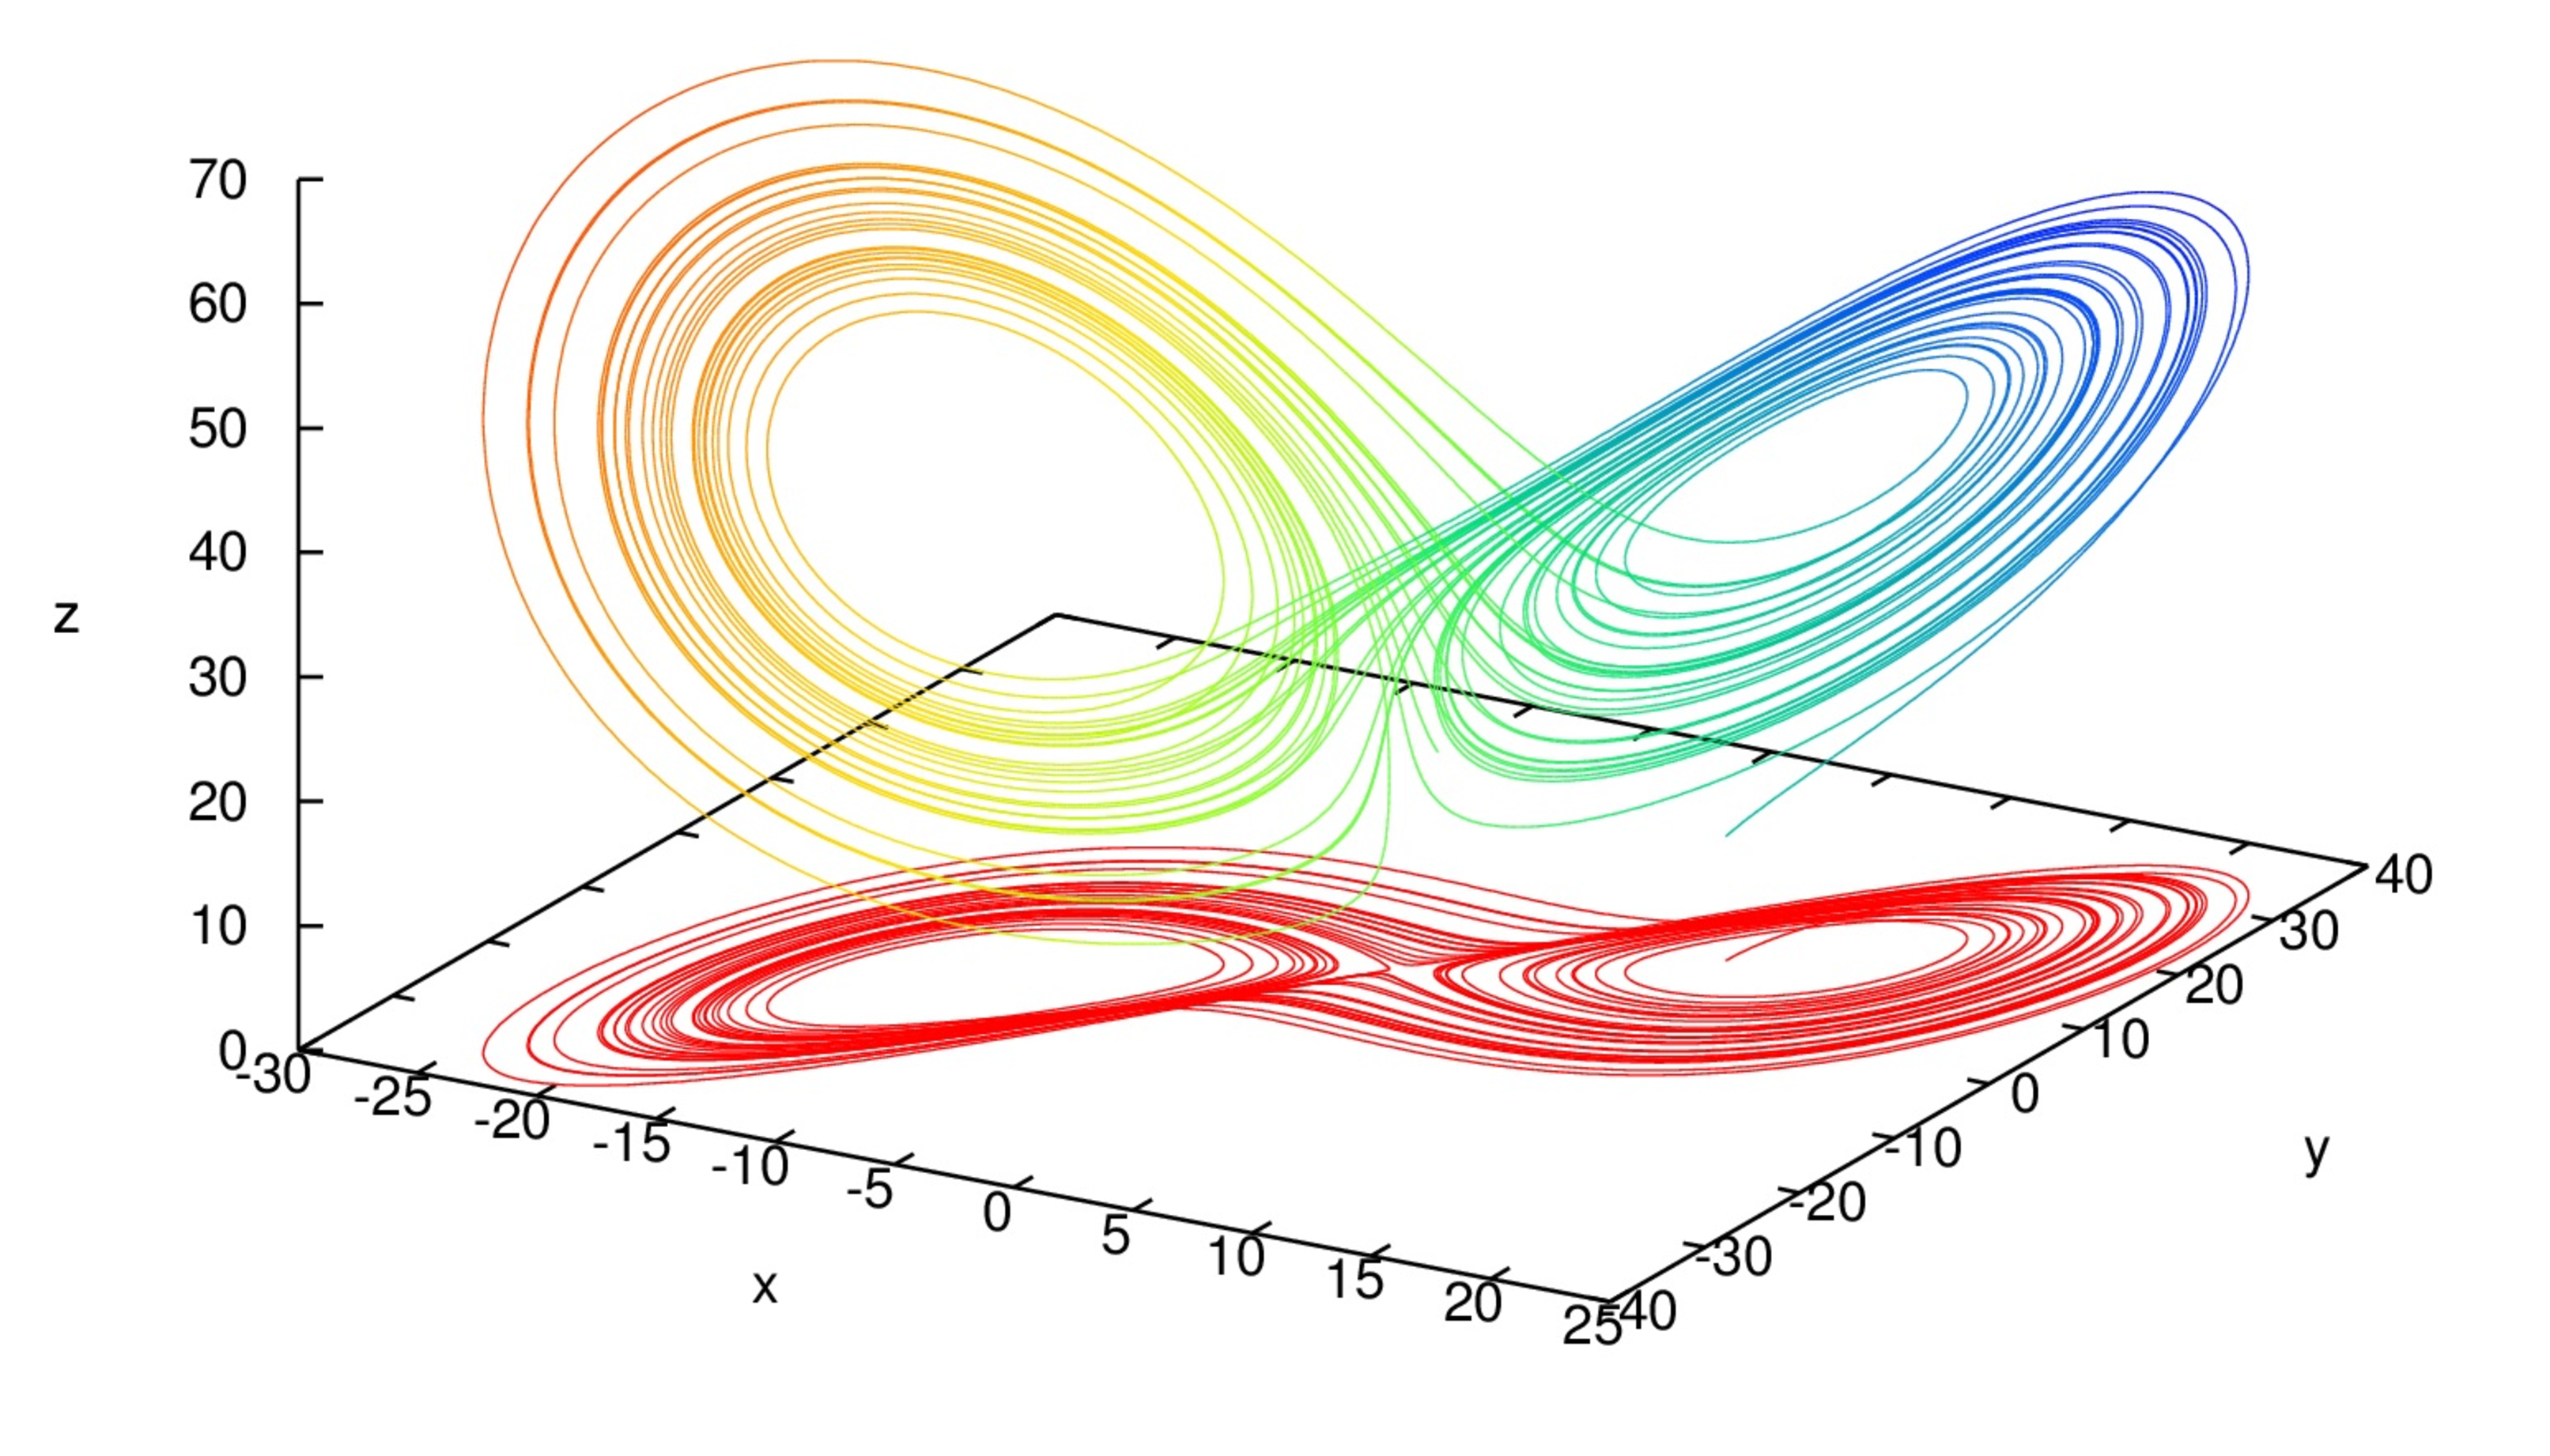
\includegraphics[width=0.9\linewidth]{9_fortran6/figs/lorenz.eps}
\caption{Lorenzアトラクター. }
\end{figure}

\subsection*{$<$演習課題5.2$>$}
\begin{enumerate}
\item $a=10, b=8/3$と固定した上で, Lorenz方程式のシミュレーションを実施せよ.
$\mu$を徐々に増加させ, どのような解が現れるか調べ, 厳密解と比較せよ. 
\item 初期値がわずかに(例えば1\%程度)異なる2ケースのシミュレーション結果を比較せよ.
\end{enumerate}


